\section{Velvet Interlinks}\label{sec:velvet}
Velvet forks, introduced by Kiayias et al.~\cite{nipopows},
were explored in depth by Zamyatin et al.~\cite{velvet}. In a
velvet fork, blocks created by upgraded miners (called \emph{velvet blocks}) are
accepted by unupgraded miners as in a soft fork. Additionally, blocks created by
unupgraded miners are also accepted by upgraded miners. This allows the protocol
to upgrade even if only a minority of miners upgrade. To maintain
backwards compatibility and avoid causing a permanent fork, the additional data included
in a block is \emph{advisory} and must be accepted whether it exists or not.
Even if the additional data is invalid or malicious, upgraded nodes
(called \emph{velvet nodes}) are \emph{forced} to accept the blocks.
It has been posited~\cite{nipopows,flyclient} that,
among other protocols, superlight client interlinking
can be deployed using a velvet fork.
The
na\"ive approach to interlink the chain with a velvet fork is to have
upgraded miners include the interlink pointer in the coinbase of the blocks they produce, but
accept blocks with missing or incorrect interlinks
(this approach was conjectured secure prior to this work~\cite{nipopows,flyclient}).
As we show in this work, the approach is susceptible to unexpected attacks. A
surgical change in the way velvet blocks are produced is necessary to achieve
security.

In a velvet fork, only a minority of honest parties needs to support the protocol
changes. We refer to this percentage as the ``velvet parameter''.

\begin{definition}[Velvet Parameter]
	The \emph{velvet parameter} $g$ is defined as the percentage of honest parties
	that have upgraded to the new protocol. The absolute number of honest upgraded
	parties is denoted $n_h$ and it holds that
	$n_h = g (n - t)$.
	\label{defn:velvet_honest_majority}
\end{definition}

Unupgraded honest nodes will produce blocks
containing no interlink, while upgraded honest nodes will produce blocks
containing truthful interlinks. Therefore, any block with invalid interlinks is
adversarial. However, such blocks cannot be rejected by the
upgraded nodes, as this gives the adversary an opportunity to cause a permanent
fork. A block generated by the adversary can thus contain arbitrary interlinks
and yet become honestly adopted. Because the honest prover is an
upgraded full node, it determines what the correct interlink pointers are by
examining the whole previous chain, and can deduce whether a block contains
invalid interlinks. In that case, the prover can simply treat such blocks as
unupgraded. In the context of the attack presented in the following
section, we examine the case where the adversary includes false interlink
pointers. We distinguish blocks based on whether they follow the velvet protocol
rules or they deviate from them.

\begin{definition}[Smooth and Thorny blocks]
A block in a velvet upgrade is called \emph{smooth} if it contains
auxiliary data corresponding to the honest upgraded protocol. A block
is called \emph{thorny} if it contains auxiliary data, but the data differs from
the honest upgraded protocol. A block is neither smooth nor thorny if it
contains no auxiliary data, while any upgraded block is either smooth or thorny.
\end{definition}

In the case of velvet forks for interlinking, the auxiliary data consists
of the interlink Merkle Tree root.

\noindent
\textbf{A na\"ive velvet scheme.}
In previous work~\cite{nipopows}, it was conjectured that superblock NIPoPoWs
remain secure under a velvet fork. We call this scheme the \emph{Na\"ive Velvet
NIPoPoW} protocol. It is similar to the NIPoPoW protocol in the
soft fork case. The na\"ive velvet NIPoPoW protocol works as follows.
Each upgraded honest miner attempts to mine a block $b$
that includes interlink pointers in the form of a Merkle Tree included in its
coinbase transaction. For each level $\mu$, the interlink contains a pointer to
the most recent among all the ancestors of $b$ that have achieved at least
level $\mu$, regardless of whether the referenced block is upgraded or not and
regardless of whether its interlinks are valid. Unupgraded honest nodes will
keep mining blocks on the chain as usual; because the status of a block as
superblock does not require it to be mined by an upgraded miner, the unupgraded
miners contribute mining power to the creation of superblocks.

The prover in the na\"ive velvet NIPoPoWs works as follows. The honest
prover constructs the proof $\pi \chi$ as in Algorithm~\ref{alg.nipopow-maxchain}.
The outstanding issue is that
$\pi$ does not form a chain because some of
its blocks may not be upgraded and they may not contain any pointers (or may
contain invalid pointers).
Suppose $\pi[i]$ is the most recent $\mu$-superblock preceding $\pi[i + 1]$.
The prover must provide a connection between $\pi[i + 1]$ and $\pi[i]$.
The block $\pi[i + 1]$ is a superblock and exists at some position $j$ in the
underlying chain $\chain$ of the prover, i.e., $\pi[i + 1] = \chain[j]$. If
$\chain[j]$ is smooth, then the interlink pointer at level $\mu$ within
it can be used. Otherwise, the prover uses the \emph{previd} pointer of
$\pi[i + 1] = \chain[j]$ to repeatedly reach the parents of $\chain[j]$, namely
$\chain[j - 1], \chain[j - 2], \cdots$ until a smooth block $b$ between $\pi[i]$
and $\pi[i + 1]$ is found in $\chain$, or until $\pi[i]$ is reached.
The block $b$ contains a pointer to
$\pi[i]$, as $\pi[i]$ is also the most recent $\mu$-superblock ancestor of $b$.
The blocks $\chain[j - 1], \chain[j - 2], \cdots, b$ are then included in the
proof to illustrate that $\pi[i]$ is an ancestor of $\pi[i + 1]$.

The (flawed) argument   why the above scheme works is as follows. First of all, the
scheme does not add many new blocks to the proof. In expectation, if a fully
honestly generated chain is processed, after in expectation $\frac{1}{g}$ blocks
have been traversed, a smooth block will be found and the connection to $\pi[i]$
will be made. Thus, the number of blocks needed in the proof increases by a
factor of $\frac{1}{g}$. Security was argued as follows: An honest party
includes in their proof as many blocks as in a soft forked NIPoPoW, albeit by
using an indirect connection. The crucial feature is that it is not missing any
superblocks. Even if the adversary creates interlinks that skip over some honest
superblocks, the honest prover will not utilize these interlinks, but will use
the ``slow route'' of level $0$ instead. The adversarial prover, on the other
hand, can only use honest interlinks as before, but may also use false
interlinks in blocks mined by the adversary. However, these false
interlinks cannot point to blocks of incorrect level. The reason is
that the verifier looks at each block hash to verify its level and
therefore cannot be cheated. The only problem a fake interlink can cause is that
it can point to a $\mu$-superblock which is not the \emph{most recent} ancestor,
but some older $\mu$-superblock ancestor in the same chain,
as illustrated in Figure~\ref{fig:skip_ancestor}. However, the adversarial
prover can only harm herself by using such pointers, as the result will
be a shorter superchain.

\begin{figure}
	\begin{center}
		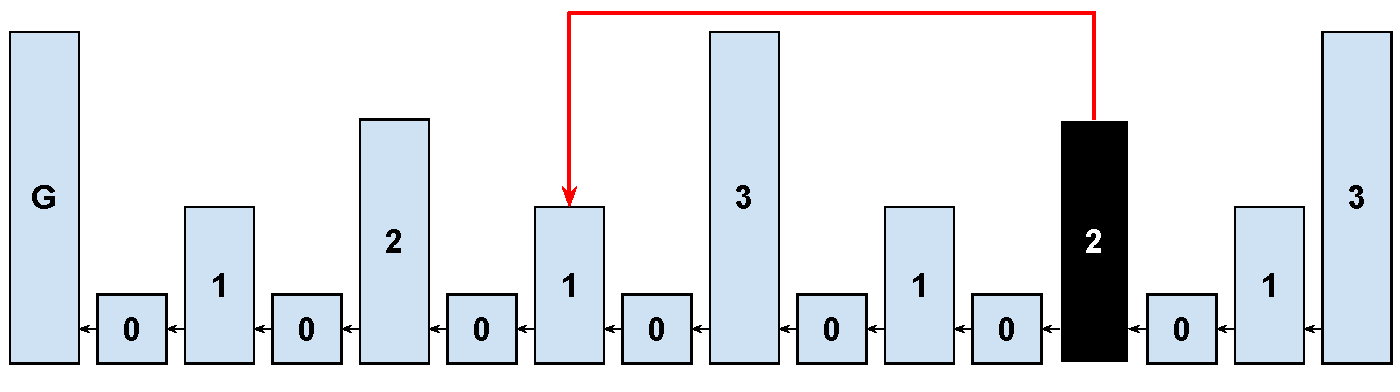
\includegraphics[width=0.8\columnwidth]{figures/simple_thorny.pdf}
	\end{center}
    \caption{A thorny pointer of an adversarial block, colored black, in an honest party's chain. The thorny block points to a $1$-superblock which is an ancestor
		$1$-superblock, but not the \emph{most recent} ancestor $1$-superblock.}
	\label{fig:skip_ancestor}
\end{figure}

We conclude that the honest verifier comparing the honest superchain
against the adversarial superchain will reach the same conclusion in a velvet
fork as he would have reached in a soft fork: Because the honest
superchain in the velvet case contains the same amount of blocks as the honest
superchain in the soft fork case, but the adversarial superchain in the velvet
case contains fewer blocks than in the soft fork case, the comparison will
remain in favor of the honest party. As we will see in the next section, this
conclusion is incorrect.
